 \subsubsection{Переход от центроплана к хвостовой части} 

\begin{figure}[h]
\centering
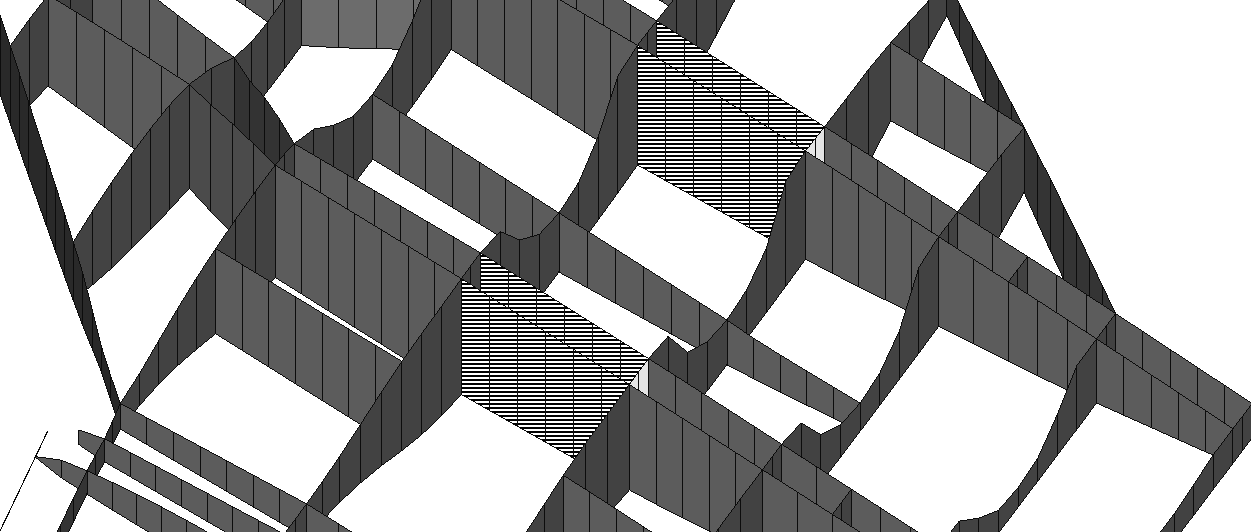
\includegraphics[width=0.8\textwidth]{IsoviewOfPantsBW}
\caption{Вид центральной части фюзеляжа с выделенными стенками}
\label{IsoviewOfPants}
\end{figure}

Для предварительной оценки НДС наиболее нагруженных деталей и узлов хвостовой части корпуса БПЛА была решена модельная задача по оценке нагруженности вертикальных стенок, обеспечивающих передачу нагрузок от двигателя, оборудования и топлива на конструкцию центроплана (стенки обозначены на Рис.~\ref{IsoviewOfPants} серой заливкой, светло-серой заливкой обозначены зоны основных узлов крепления двигателя). Уровень нагружения был оценен на основе аналитических формул. Схема нагружения модельных стенок показана на Рис.\ref{IsoviewOfPantsModel}.

\begin{figure}[H]
\centering
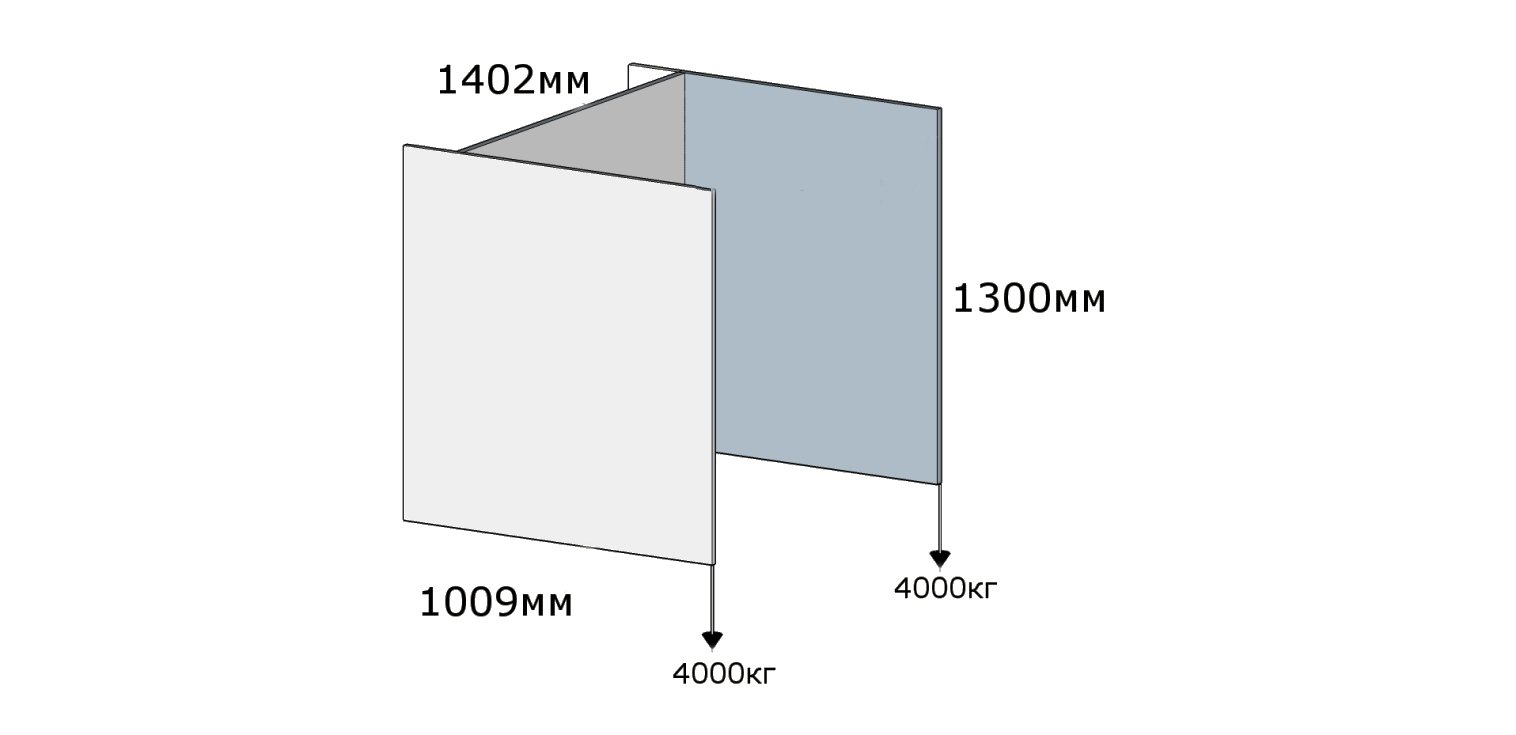
\includegraphics[width=0.8\textwidth]{IsoviewOfPantsModel}
\caption{Схема нагружения модельных стенок}
\label{IsoviewOfPantsModel}
\end{figure}


Уровень нагружения оценивался по величинам касательных напряжений. Касательные напряжения в пластине при чистом сдвиге равны

\begin{equation}
\tau=\frac{3}{2}\cdot\frac{Q}{bh}
\end{equation}
Критические по устойчивости касательные напряжения в пластине при чистом сдвиге равны \cite{Volmir}:

\begin{equation}
\tau_\text{кр}=\frac{K}{12}\frac{\pi^2D}{b^2h} = \frac{K}{12}\frac{\pi^2E}{(1-\mu^2)}\left(\frac{h}{b}\right)^2,\, K=5.34 + 4\frac{a}{b},
\end{equation}
где $a$ - размер пластины вдоль направления действия силы, $b$ - размер пластины поперек направления действия силы, $h$ - толщина пластины, $D$ - изгибная жесткость пластины, $E$ - модуль Юнга, $\mu$ - модуль Пуассона материала пластины, $Q$ - приложенная сила.
Допускаемые толщины найдем из условия

\begin{equation}
\tau_\text{кр} \geq \tau \to h \geq \sqrt[3]{\frac{3\cdot12}{2}\frac{Qb\cdot(1-\mu^2)}{k\pi^2E}} 
\end{equation}
Подставляя значения, получим:

\begin{equation}
Q=\frac{8000}{n}\text{кгс},\,a=1300\text{мм},\,b=1009\text{мм},\,\mu=0.3,\,E=7000\frac{\text{кгс}}{\text{мм}^2}
\end{equation}

\begin{equation}
h \geq \sqrt[3]{\frac{18\cdot8000\cdot1000\cdot(1-\mu^2)}{k\pi^2En}} = \frac{5.67}{\sqrt[3]{n}} 
\end{equation}

Таким образом, для случаев $n = 2$ и $n = 4$  были получены минимальные допустимые толщины, 
равные

\begin{equation}
h\geq4.50\text{мм},\,n=2
\end{equation}
\begin{equation}
h\geq2.83\text{мм},\,n=4
\end{equation}